\documentclass[twoside]{book}

% Packages required by doxygen
\usepackage{fixltx2e}
\usepackage{calc}
\usepackage{doxygen}
\usepackage[export]{adjustbox} % also loads graphicx
\usepackage{graphicx}
\usepackage[utf8]{inputenc}
\usepackage{makeidx}
\usepackage{multicol}
\usepackage{multirow}
\PassOptionsToPackage{warn}{textcomp}
\usepackage{textcomp}
\usepackage[nointegrals]{wasysym}
\usepackage[table]{xcolor}

% NLS support packages
\usepackage[spanish]{babel}
% Font selection
\usepackage[T1]{fontenc}
\usepackage[scaled=.90]{helvet}
\usepackage{courier}
\usepackage{amssymb}
\usepackage{sectsty}
\renewcommand{\familydefault}{\sfdefault}
\allsectionsfont{%
  \fontseries{bc}\selectfont%
  \color{darkgray}%
}
\renewcommand{\DoxyLabelFont}{%
  \fontseries{bc}\selectfont%
  \color{darkgray}%
}
\newcommand{\+}{\discretionary{\mbox{\scriptsize$\hookleftarrow$}}{}{}}

% Page & text layout
\usepackage{geometry}
\geometry{%
  a4paper,%
  top=2.5cm,%
  bottom=2.5cm,%
  left=2.5cm,%
  right=2.5cm%
}
\tolerance=750
\hfuzz=15pt
\hbadness=750
\setlength{\emergencystretch}{15pt}
\setlength{\parindent}{0cm}
\setlength{\parskip}{3ex plus 2ex minus 2ex}
\makeatletter
\renewcommand{\paragraph}{%
  \@startsection{paragraph}{4}{0ex}{-1.0ex}{1.0ex}{%
    \normalfont\normalsize\bfseries\SS@parafont%
  }%
}
\renewcommand{\subparagraph}{%
  \@startsection{subparagraph}{5}{0ex}{-1.0ex}{1.0ex}{%
    \normalfont\normalsize\bfseries\SS@subparafont%
  }%
}
\makeatother

% Headers & footers
\usepackage{fancyhdr}
\pagestyle{fancyplain}
\fancyhead[LE]{\fancyplain{}{\bfseries\thepage}}
\fancyhead[CE]{\fancyplain{}{}}
\fancyhead[RE]{\fancyplain{}{\bfseries\leftmark}}
\fancyhead[LO]{\fancyplain{}{\bfseries\rightmark}}
\fancyhead[CO]{\fancyplain{}{}}
\fancyhead[RO]{\fancyplain{}{\bfseries\thepage}}
\fancyfoot[LE]{\fancyplain{}{}}
\fancyfoot[CE]{\fancyplain{}{}}
\fancyfoot[RE]{\fancyplain{}{\bfseries\scriptsize Generado por Doxygen }}
\fancyfoot[LO]{\fancyplain{}{\bfseries\scriptsize Generado por Doxygen }}
\fancyfoot[CO]{\fancyplain{}{}}
\fancyfoot[RO]{\fancyplain{}{}}
\renewcommand{\footrulewidth}{0.4pt}
\renewcommand{\chaptermark}[1]{%
  \markboth{#1}{}%
}
\renewcommand{\sectionmark}[1]{%
  \markright{\thesection\ #1}%
}

% Indices & bibliography
\usepackage{natbib}
\usepackage[titles]{tocloft}
\setcounter{tocdepth}{3}
\setcounter{secnumdepth}{5}
\makeindex

% Hyperlinks (required, but should be loaded last)
\usepackage{ifpdf}
\ifpdf
  \usepackage[pdftex,pagebackref=true]{hyperref}
\else
  \usepackage[ps2pdf,pagebackref=true]{hyperref}
\fi
\hypersetup{%
  colorlinks=true,%
  linkcolor=blue,%
  citecolor=blue,%
  unicode%
}

% Custom commands
\newcommand{\clearemptydoublepage}{%
  \newpage{\pagestyle{empty}\cleardoublepage}%
}

\usepackage{caption}
\captionsetup{labelsep=space,justification=centering,font={bf},singlelinecheck=off,skip=4pt,position=top}

%===== C O N T E N T S =====

\begin{document}

% Titlepage & ToC
\hypersetup{pageanchor=false,
             bookmarksnumbered=true,
             pdfencoding=unicode
            }
\pagenumbering{alph}
\begin{titlepage}
\vspace*{7cm}
\begin{center}%
{\Large Grafo-\/\+Dijkstra\+\_\+\+Server \\[1ex]\large 1.\+0 }\\
\vspace*{1cm}
{\large Generado por Doxygen 1.8.13}\\
\end{center}
\end{titlepage}
\clearemptydoublepage
\pagenumbering{roman}
\tableofcontents
\clearemptydoublepage
\pagenumbering{arabic}
\hypersetup{pageanchor=true}

%--- Begin generated contents ---
\chapter{Grafo-\/\+Dijkstra\+\_\+\+Server}
\label{md__r_e_a_d_m_e}
\Hypertarget{md__r_e_a_d_m_e}
\input{md__r_e_a_d_m_e}
\chapter{Indice jerárquico}
\section{Class Hierarchy}
This inheritance list is sorted roughly, but not completely, alphabetically\+:\begin{DoxyCompactList}
\item \contentsline{section}{Grafo}{\pageref{class_grafo}}{}
\item Q\+Tcp\+Server\begin{DoxyCompactList}
\item \contentsline{section}{Dijkstra\+Server}{\pageref{class_dijkstra_server}}{}
\end{DoxyCompactList}
\item Q\+Tcp\+Socket\begin{DoxyCompactList}
\item \contentsline{section}{Dijkstra\+Socket}{\pageref{class_dijkstra_socket}}{}
\end{DoxyCompactList}
\end{DoxyCompactList}

\chapter{Índice de clases}
\section{Class List}
Here are the classes, structs, unions and interfaces with brief descriptions\+:\begin{DoxyCompactList}
\item\contentsline{section}{\hyperlink{class_dijkstra_server}{Dijkstra\+Server} }{\pageref{class_dijkstra_server}}{}
\item\contentsline{section}{\hyperlink{class_dijkstra_socket}{Dijkstra\+Socket} }{\pageref{class_dijkstra_socket}}{}
\item\contentsline{section}{\hyperlink{class_grafo}{Grafo} }{\pageref{class_grafo}}{}
\end{DoxyCompactList}

\chapter{Indice de archivos}
\section{File List}
Here is a list of all files with brief descriptions\+:\begin{DoxyCompactList}
\item\contentsline{section}{\hyperlink{dijkstraserver_8cpp}{dijkstraserver.\+cpp} }{\pageref{dijkstraserver_8cpp}}{}
\item\contentsline{section}{\hyperlink{dijkstraserver_8h}{dijkstraserver.\+h} \\*Extiende de Q\+Tcp\+Server y contiene la lógica para comunicar al cliente con la implementación del grafo }{\pageref{dijkstraserver_8h}}{}
\item\contentsline{section}{\hyperlink{dijkstrasocket_8cpp}{dijkstrasocket.\+cpp} }{\pageref{dijkstrasocket_8cpp}}{}
\item\contentsline{section}{\hyperlink{dijkstrasocket_8h}{dijkstrasocket.\+h} \\*Extiende de Q\+Tcp\+Sockety contiene la lógica para comunicar al cliente con la implementación del grafo }{\pageref{dijkstrasocket_8h}}{}
\item\contentsline{section}{\hyperlink{grafo_8cpp}{grafo.\+cpp} }{\pageref{grafo_8cpp}}{}
\item\contentsline{section}{\hyperlink{grafo_8h}{grafo.\+h} \\*Contiene un grafo y la función Dijkstra }{\pageref{grafo_8h}}{}
\item\contentsline{section}{\hyperlink{main_8cpp}{main.\+cpp} }{\pageref{main_8cpp}}{}
\end{DoxyCompactList}

\chapter{Documentación de las clases}
\hypertarget{class_dijkstra_server}{}\section{Referencia de la Clase Dijkstra\+Server}
\label{class_dijkstra_server}\index{Dijkstra\+Server@{Dijkstra\+Server}}


{\ttfamily \#include $<$dijkstraserver.\+h$>$}



Diagrama de herencias de Dijkstra\+Server
\nopagebreak
\begin{figure}[H]
\begin{center}
\leavevmode
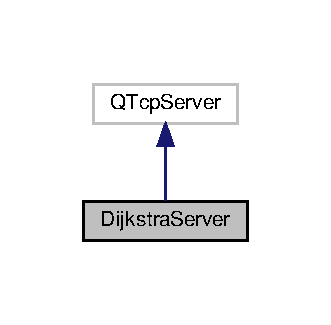
\includegraphics[width=159pt]{class_dijkstra_server__inherit__graph}
\end{center}
\end{figure}


Diagrama de colaboración para Dijkstra\+Server\+:
\nopagebreak
\begin{figure}[H]
\begin{center}
\leavevmode
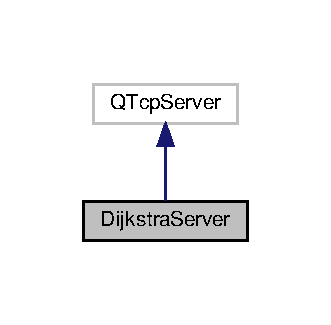
\includegraphics[width=159pt]{class_dijkstra_server__coll__graph}
\end{center}
\end{figure}
\subsection*{Métodos públicos}
\begin{DoxyCompactItemize}
\item 
\hyperlink{class_dijkstra_server_a9c8106e2267967439928ef48b2a66660}{Dijkstra\+Server} (Q\+Object $\ast$parent=nullptr)
\begin{DoxyCompactList}\small\item\em Constructor de \hyperlink{class_dijkstra_server}{Dijkstra\+Server}. \end{DoxyCompactList}\item 
bool \hyperlink{class_dijkstra_server_ad285a85f623398d6feffbfd138e4c76d}{start\+Server} (quint16 port)
\begin{DoxyCompactList}\small\item\em Inicia el servidor. \end{DoxyCompactList}\end{DoxyCompactItemize}
\subsection*{Métodos protegidos}
\begin{DoxyCompactItemize}
\item 
void \hyperlink{class_dijkstra_server_aab86d4d415a39981088e75a140cfd6d4}{incoming\+Connection} (qintptr handle)
\begin{DoxyCompactList}\small\item\em Llamada por el servidor cuando hay una nueva conexión disponible, reimplementado de Q\+Tcp\+Server. \end{DoxyCompactList}\end{DoxyCompactItemize}


\subsection{Documentación del constructor y destructor}
\mbox{\Hypertarget{class_dijkstra_server_a9c8106e2267967439928ef48b2a66660}\label{class_dijkstra_server_a9c8106e2267967439928ef48b2a66660}} 
\index{Dijkstra\+Server@{Dijkstra\+Server}!Dijkstra\+Server@{Dijkstra\+Server}}
\index{Dijkstra\+Server@{Dijkstra\+Server}!Dijkstra\+Server@{Dijkstra\+Server}}
\subsubsection{\texorpdfstring{Dijkstra\+Server()}{DijkstraServer()}}
{\footnotesize\ttfamily Dijkstra\+Server\+::\+Dijkstra\+Server (\begin{DoxyParamCaption}\item[{Q\+Object $\ast$}]{parent = {\ttfamily nullptr} }\end{DoxyParamCaption})}



Constructor de \hyperlink{class_dijkstra_server}{Dijkstra\+Server}. 


\begin{DoxyParams}{Parámetros}
{\em parent} & \\
\hline
\end{DoxyParams}


\subsection{Documentación de las funciones miembro}
\mbox{\Hypertarget{class_dijkstra_server_aab86d4d415a39981088e75a140cfd6d4}\label{class_dijkstra_server_aab86d4d415a39981088e75a140cfd6d4}} 
\index{Dijkstra\+Server@{Dijkstra\+Server}!incoming\+Connection@{incoming\+Connection}}
\index{incoming\+Connection@{incoming\+Connection}!Dijkstra\+Server@{Dijkstra\+Server}}
\subsubsection{\texorpdfstring{incoming\+Connection()}{incomingConnection()}}
{\footnotesize\ttfamily void Dijkstra\+Server\+::incoming\+Connection (\begin{DoxyParamCaption}\item[{qintptr}]{handle }\end{DoxyParamCaption})\hspace{0.3cm}{\ttfamily [protected]}}



Llamada por el servidor cuando hay una nueva conexión disponible, reimplementado de Q\+Tcp\+Server. 


\begin{DoxyParams}{Parámetros}
{\em handle} & del socket que envia la señal \\
\hline
\end{DoxyParams}
\mbox{\Hypertarget{class_dijkstra_server_ad285a85f623398d6feffbfd138e4c76d}\label{class_dijkstra_server_ad285a85f623398d6feffbfd138e4c76d}} 
\index{Dijkstra\+Server@{Dijkstra\+Server}!start\+Server@{start\+Server}}
\index{start\+Server@{start\+Server}!Dijkstra\+Server@{Dijkstra\+Server}}
\subsubsection{\texorpdfstring{start\+Server()}{startServer()}}
{\footnotesize\ttfamily bool Dijkstra\+Server\+::start\+Server (\begin{DoxyParamCaption}\item[{quint16}]{port }\end{DoxyParamCaption})}



Inicia el servidor. 


\begin{DoxyParams}{Parámetros}
{\em Puerto} & en donde se desea iniciar el servidor \\
\hline
\end{DoxyParams}
\begin{DoxyReturn}{Devuelve}
Booleano true si se logró iniciar el servidor, false si no se logró 
\end{DoxyReturn}


La documentación para esta clase fue generada a partir de los siguientes ficheros\+:\begin{DoxyCompactItemize}
\item 
\hyperlink{dijkstraserver_8h}{dijkstraserver.\+h}\item 
\hyperlink{dijkstraserver_8cpp}{dijkstraserver.\+cpp}\end{DoxyCompactItemize}

\hypertarget{class_dijkstra_socket}{}\section{Referencia de la Clase Dijkstra\+Socket}
\label{class_dijkstra_socket}\index{Dijkstra\+Socket@{Dijkstra\+Socket}}


{\ttfamily \#include $<$dijkstrasocket.\+h$>$}



Diagrama de herencias de Dijkstra\+Socket
\nopagebreak
\begin{figure}[H]
\begin{center}
\leavevmode
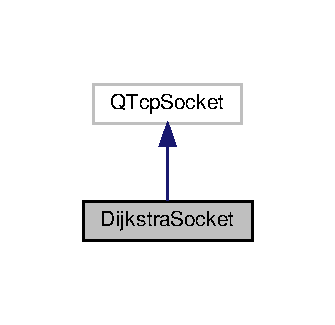
\includegraphics[width=161pt]{class_dijkstra_socket__inherit__graph}
\end{center}
\end{figure}


Diagrama de colaboración para Dijkstra\+Socket\+:
\nopagebreak
\begin{figure}[H]
\begin{center}
\leavevmode
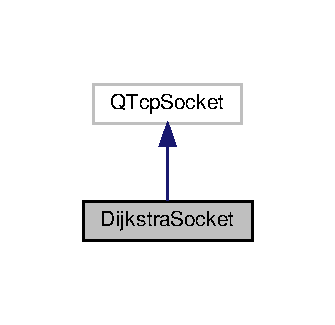
\includegraphics[width=161pt]{class_dijkstra_socket__coll__graph}
\end{center}
\end{figure}
\subsection*{Señales}
\begin{DoxyCompactItemize}
\item 
void \hyperlink{class_dijkstra_socket_ad942276d377f42992ac9dfd5fe32219c}{Dijkstra\+Ready\+Read} (\hyperlink{class_dijkstra_socket}{Dijkstra\+Socket} $\ast$)
\item 
void \hyperlink{class_dijkstra_socket_a4527ae22be46f923b0c13eabf170e96f}{Dijkstra\+State\+Changed} (\hyperlink{class_dijkstra_socket}{Dijkstra\+Socket} $\ast$, int)
\end{DoxyCompactItemize}
\subsection*{Métodos públicos}
\begin{DoxyCompactItemize}
\item 
\hyperlink{class_dijkstra_socket_ab788220c12a6f985d5b036d69205b5e6}{Dijkstra\+Socket} (qintptr handle, Q\+Object $\ast$parent=nullptr)
\end{DoxyCompactItemize}


\subsection{Documentación del constructor y destructor}
\mbox{\Hypertarget{class_dijkstra_socket_ab788220c12a6f985d5b036d69205b5e6}\label{class_dijkstra_socket_ab788220c12a6f985d5b036d69205b5e6}} 
\index{Dijkstra\+Socket@{Dijkstra\+Socket}!Dijkstra\+Socket@{Dijkstra\+Socket}}
\index{Dijkstra\+Socket@{Dijkstra\+Socket}!Dijkstra\+Socket@{Dijkstra\+Socket}}
\subsubsection{\texorpdfstring{Dijkstra\+Socket()}{DijkstraSocket()}}
{\footnotesize\ttfamily Dijkstra\+Socket\+::\+Dijkstra\+Socket (\begin{DoxyParamCaption}\item[{qintptr}]{handle,  }\item[{Q\+Object $\ast$}]{parent = {\ttfamily nullptr} }\end{DoxyParamCaption})}



\subsection{Documentación de las funciones miembro}
\mbox{\Hypertarget{class_dijkstra_socket_ad942276d377f42992ac9dfd5fe32219c}\label{class_dijkstra_socket_ad942276d377f42992ac9dfd5fe32219c}} 
\index{Dijkstra\+Socket@{Dijkstra\+Socket}!Dijkstra\+Ready\+Read@{Dijkstra\+Ready\+Read}}
\index{Dijkstra\+Ready\+Read@{Dijkstra\+Ready\+Read}!Dijkstra\+Socket@{Dijkstra\+Socket}}
\subsubsection{\texorpdfstring{Dijkstra\+Ready\+Read}{DijkstraReadyRead}}
{\footnotesize\ttfamily void Dijkstra\+Socket\+::\+Dijkstra\+Ready\+Read (\begin{DoxyParamCaption}\item[{\hyperlink{class_dijkstra_socket}{Dijkstra\+Socket} $\ast$}]{ }\end{DoxyParamCaption})\hspace{0.3cm}{\ttfamily [signal]}}

\mbox{\Hypertarget{class_dijkstra_socket_a4527ae22be46f923b0c13eabf170e96f}\label{class_dijkstra_socket_a4527ae22be46f923b0c13eabf170e96f}} 
\index{Dijkstra\+Socket@{Dijkstra\+Socket}!Dijkstra\+State\+Changed@{Dijkstra\+State\+Changed}}
\index{Dijkstra\+State\+Changed@{Dijkstra\+State\+Changed}!Dijkstra\+Socket@{Dijkstra\+Socket}}
\subsubsection{\texorpdfstring{Dijkstra\+State\+Changed}{DijkstraStateChanged}}
{\footnotesize\ttfamily void Dijkstra\+Socket\+::\+Dijkstra\+State\+Changed (\begin{DoxyParamCaption}\item[{\hyperlink{class_dijkstra_socket}{Dijkstra\+Socket} $\ast$}]{,  }\item[{int}]{ }\end{DoxyParamCaption})\hspace{0.3cm}{\ttfamily [signal]}}



La documentación para esta clase fue generada a partir de los siguientes ficheros\+:\begin{DoxyCompactItemize}
\item 
\hyperlink{dijkstrasocket_8h}{dijkstrasocket.\+h}\item 
\hyperlink{dijkstrasocket_8cpp}{dijkstrasocket.\+cpp}\end{DoxyCompactItemize}

\hypertarget{class_grafo}{}\section{Grafo Class Reference}
\label{class_grafo}\index{Grafo@{Grafo}}


{\ttfamily \#include $<$grafo.\+h$>$}

\subsection*{Public Member Functions}
\begin{DoxyCompactItemize}
\item 
\hyperlink{class_grafo_ab810bbe26a98e9af6661ccddff66b03b}{Grafo} ()
\begin{DoxyCompactList}\small\item\em Constructor de \hyperlink{class_grafo}{Grafo}. \end{DoxyCompactList}\item 
\hyperlink{class_grafo_a16f3fbba0de2667dfba3b657cb7e95ff}{$\sim$\+Grafo} ()
\begin{DoxyCompactList}\small\item\em Destructor de \hyperlink{class_grafo}{Grafo}. \end{DoxyCompactList}\item 
Q\+String \hyperlink{class_grafo_a8fe931a9a154866add1bf763dcb88c12}{dijkstra} (int startnode, int endnode)
\begin{DoxyCompactList}\small\item\em dijkstra obtiene la distancia más corta entre dos nodos \end{DoxyCompactList}\end{DoxyCompactItemize}


\subsection{Constructor \& Destructor Documentation}
\mbox{\Hypertarget{class_grafo_ab810bbe26a98e9af6661ccddff66b03b}\label{class_grafo_ab810bbe26a98e9af6661ccddff66b03b}} 
\index{Grafo@{Grafo}!Grafo@{Grafo}}
\index{Grafo@{Grafo}!Grafo@{Grafo}}
\subsubsection{\texorpdfstring{Grafo()}{Grafo()}}
{\footnotesize\ttfamily Grafo\+::\+Grafo (\begin{DoxyParamCaption}{ }\end{DoxyParamCaption})}



Constructor de \hyperlink{class_grafo}{Grafo}. 

\mbox{\Hypertarget{class_grafo_a16f3fbba0de2667dfba3b657cb7e95ff}\label{class_grafo_a16f3fbba0de2667dfba3b657cb7e95ff}} 
\index{Grafo@{Grafo}!````~Grafo@{$\sim$\+Grafo}}
\index{````~Grafo@{$\sim$\+Grafo}!Grafo@{Grafo}}
\subsubsection{\texorpdfstring{$\sim$\+Grafo()}{~Grafo()}}
{\footnotesize\ttfamily Grafo\+::$\sim$\+Grafo (\begin{DoxyParamCaption}{ }\end{DoxyParamCaption})}



Destructor de \hyperlink{class_grafo}{Grafo}. 



\subsection{Member Function Documentation}
\mbox{\Hypertarget{class_grafo_a8fe931a9a154866add1bf763dcb88c12}\label{class_grafo_a8fe931a9a154866add1bf763dcb88c12}} 
\index{Grafo@{Grafo}!dijkstra@{dijkstra}}
\index{dijkstra@{dijkstra}!Grafo@{Grafo}}
\subsubsection{\texorpdfstring{dijkstra()}{dijkstra()}}
{\footnotesize\ttfamily Q\+String Grafo\+::dijkstra (\begin{DoxyParamCaption}\item[{int}]{startnode,  }\item[{int}]{endnode }\end{DoxyParamCaption})}



dijkstra obtiene la distancia más corta entre dos nodos 


\begin{DoxyParams}{Parameters}
{\em startnode,el} & nodo inicial \\
\hline
{\em endnode,el} & nodo final \\
\hline
\end{DoxyParams}
\begin{DoxyReturn}{Returns}
Qstring con la solución, el camino y el peso total de este 
\end{DoxyReturn}


The documentation for this class was generated from the following files\+:\begin{DoxyCompactItemize}
\item 
\hyperlink{grafo_8h}{grafo.\+h}\item 
\hyperlink{grafo_8cpp}{grafo.\+cpp}\end{DoxyCompactItemize}

\chapter{Documentación de archivos}
\hypertarget{dijkstraserver_8cpp}{}\section{Referencia del Archivo dijkstraserver.\+cpp}
\label{dijkstraserver_8cpp}\index{dijkstraserver.\+cpp@{dijkstraserver.\+cpp}}
{\ttfamily \#include \char`\"{}dijkstraserver.\+h\char`\"{}}\newline
{\ttfamily \#include \char`\"{}dijkstrasocket.\+h\char`\"{}}\newline
{\ttfamily \#include $<$Q\+Text\+Stream$>$}\newline
{\ttfamily \#include $<$iostream$>$}\newline
{\ttfamily \#include $<$Q\+Debug$>$}\newline
Dependencia gráfica adjunta para dijkstraserver.\+cpp\+:
\nopagebreak
\begin{figure}[H]
\begin{center}
\leavevmode
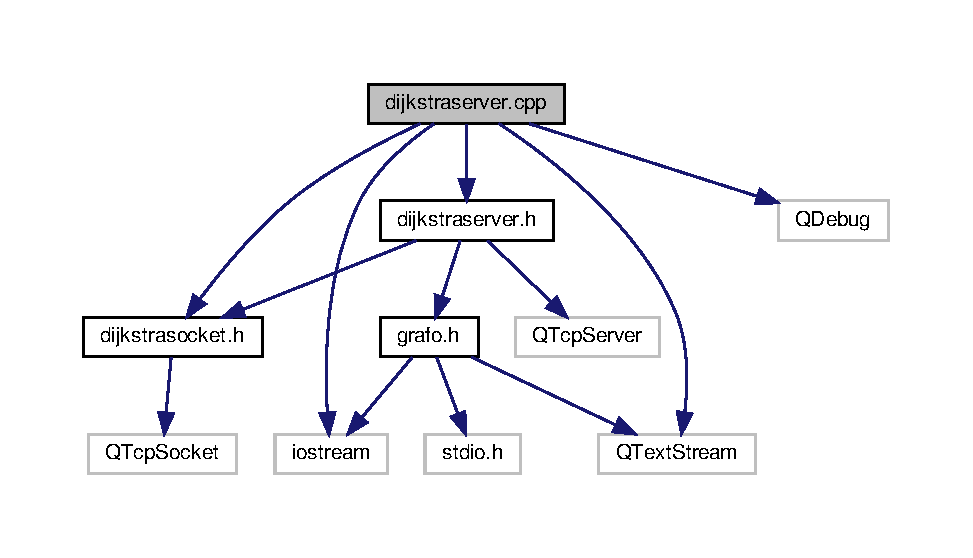
\includegraphics[width=350pt]{dijkstraserver_8cpp__incl}
\end{center}
\end{figure}

\hypertarget{dijkstraserver_8h}{}\section{Referencia del Archivo dijkstraserver.\+h}
\label{dijkstraserver_8h}\index{dijkstraserver.\+h@{dijkstraserver.\+h}}


Extiende de Q\+Tcp\+Server y contiene la lógica para comunicar al cliente con la implementación del grafo.  


{\ttfamily \#include $<$Q\+Tcp\+Server$>$}\newline
{\ttfamily \#include \char`\"{}dijkstrasocket.\+h\char`\"{}}\newline
{\ttfamily \#include \char`\"{}grafo.\+h\char`\"{}}\newline
Dependencia gráfica adjunta para dijkstraserver.\+h\+:
\nopagebreak
\begin{figure}[H]
\begin{center}
\leavevmode
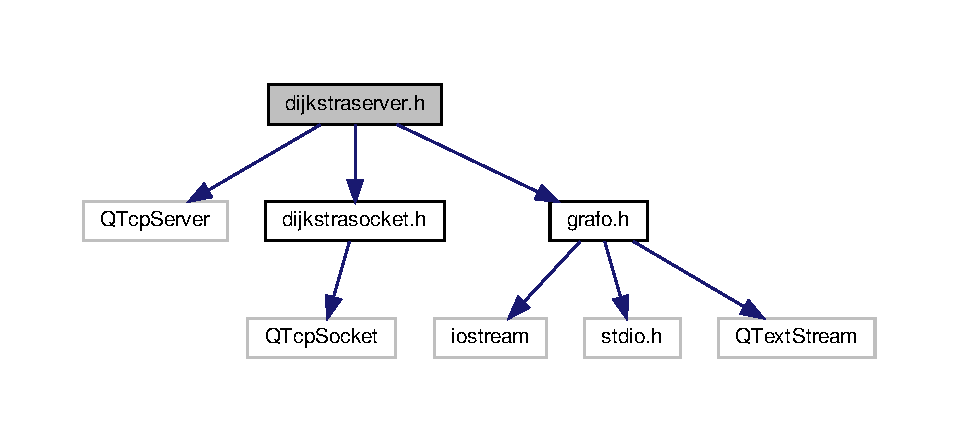
\includegraphics[width=350pt]{dijkstraserver_8h__incl}
\end{center}
\end{figure}
Gráfico de los archivos que directa o indirectamente incluyen a este archivo\+:
\nopagebreak
\begin{figure}[H]
\begin{center}
\leavevmode
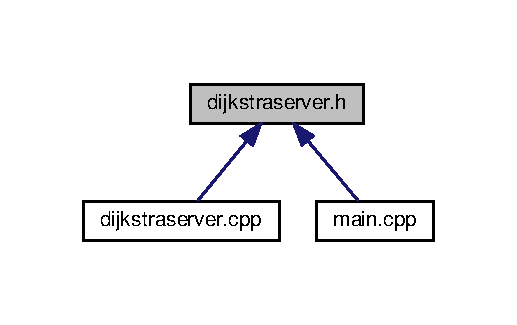
\includegraphics[width=248pt]{dijkstraserver_8h__dep__incl}
\end{center}
\end{figure}
\subsection*{Clases}
\begin{DoxyCompactItemize}
\item 
class \hyperlink{class_dijkstra_server}{Dijkstra\+Server}
\end{DoxyCompactItemize}


\subsection{Descripción detallada}
Extiende de Q\+Tcp\+Server y contiene la lógica para comunicar al cliente con la implementación del grafo. 

Dijkstra Server \begin{DoxyVersion}{Versión}
1.\+0 
\end{DoxyVersion}
\begin{DoxyAuthor}{Autor}
Jose\+Sol 
\end{DoxyAuthor}
\begin{DoxyDate}{Fecha}
02/03/2020 
\end{DoxyDate}

\hypertarget{dijkstrasocket_8cpp}{}\section{dijkstrasocket.\+cpp File Reference}
\label{dijkstrasocket_8cpp}\index{dijkstrasocket.\+cpp@{dijkstrasocket.\+cpp}}
{\ttfamily \#include \char`\"{}dijkstrasocket.\+h\char`\"{}}\newline
Include dependency graph for dijkstrasocket.\+cpp\+:
\nopagebreak
\begin{figure}[H]
\begin{center}
\leavevmode
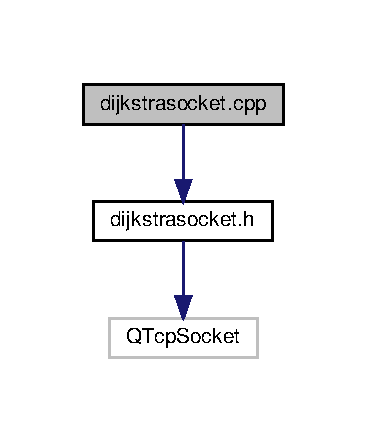
\includegraphics[width=176pt]{dijkstrasocket_8cpp__incl}
\end{center}
\end{figure}

\hypertarget{dijkstrasocket_8h}{}\section{dijkstrasocket.\+h File Reference}
\label{dijkstrasocket_8h}\index{dijkstrasocket.\+h@{dijkstrasocket.\+h}}


Extiende de Q\+Tcp\+Sockety contiene la lógica para comunicar al cliente con la implementación del grafo.  


{\ttfamily \#include $<$Q\+Tcp\+Socket$>$}\newline
Include dependency graph for dijkstrasocket.\+h\+:
\nopagebreak
\begin{figure}[H]
\begin{center}
\leavevmode
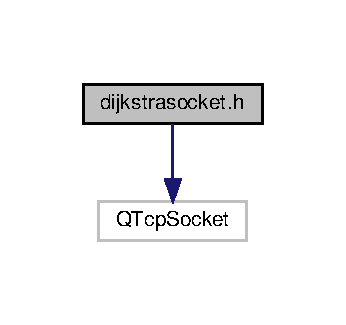
\includegraphics[width=166pt]{dijkstrasocket_8h__incl}
\end{center}
\end{figure}
This graph shows which files directly or indirectly include this file\+:
\nopagebreak
\begin{figure}[H]
\begin{center}
\leavevmode
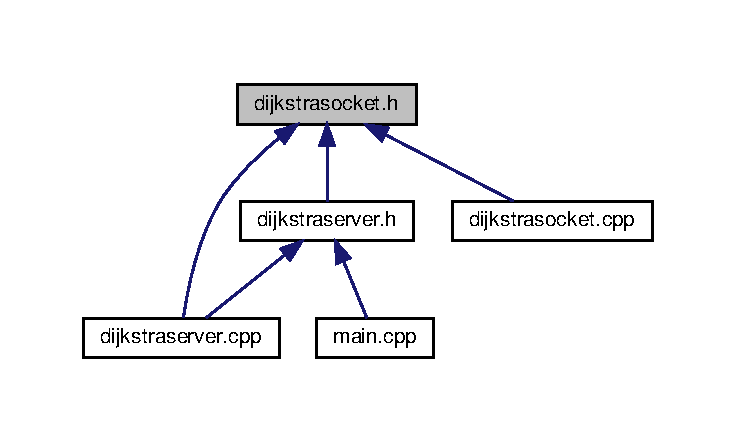
\includegraphics[width=350pt]{dijkstrasocket_8h__dep__incl}
\end{center}
\end{figure}
\subsection*{Classes}
\begin{DoxyCompactItemize}
\item 
class \hyperlink{class_dijkstra_socket}{Dijkstra\+Socket}
\end{DoxyCompactItemize}


\subsection{Detailed Description}
Extiende de Q\+Tcp\+Sockety contiene la lógica para comunicar al cliente con la implementación del grafo. 

Dijkstra Socket \begin{DoxyVersion}{Version}
1.\+0 
\end{DoxyVersion}
\begin{DoxyAuthor}{Author}
Jose\+Sol 
\end{DoxyAuthor}
\begin{DoxyDate}{Date}
02/03/2020 
\end{DoxyDate}

\hypertarget{grafo_8cpp}{}\section{Referencia del Archivo grafo.\+cpp}
\label{grafo_8cpp}\index{grafo.\+cpp@{grafo.\+cpp}}
{\ttfamily \#include \char`\"{}grafo.\+h\char`\"{}}\newline
{\ttfamily \#include $<$Q\+Text\+Stream$>$}\newline
{\ttfamily \#include $<$iostream$>$}\newline
Dependencia gráfica adjunta para grafo.\+cpp\+:
\nopagebreak
\begin{figure}[H]
\begin{center}
\leavevmode
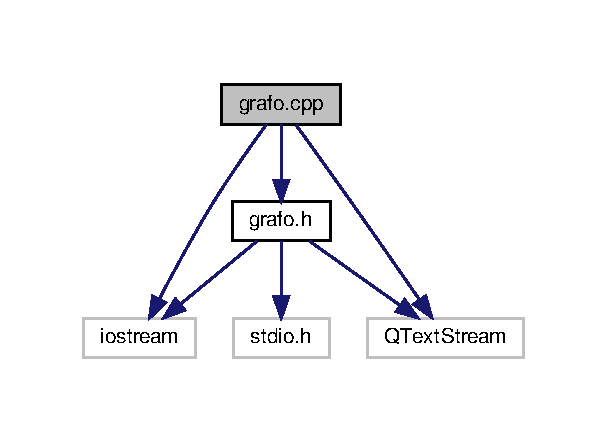
\includegraphics[width=292pt]{grafo_8cpp__incl}
\end{center}
\end{figure}

\hypertarget{grafo_8h}{}\section{grafo.\+h File Reference}
\label{grafo_8h}\index{grafo.\+h@{grafo.\+h}}


Contiene un grafo y la función Dijkstra.  


{\ttfamily \#include $<$iostream$>$}\newline
{\ttfamily \#include $<$stdio.\+h$>$}\newline
{\ttfamily \#include $<$Q\+Text\+Stream$>$}\newline
Include dependency graph for grafo.\+h\+:
\nopagebreak
\begin{figure}[H]
\begin{center}
\leavevmode
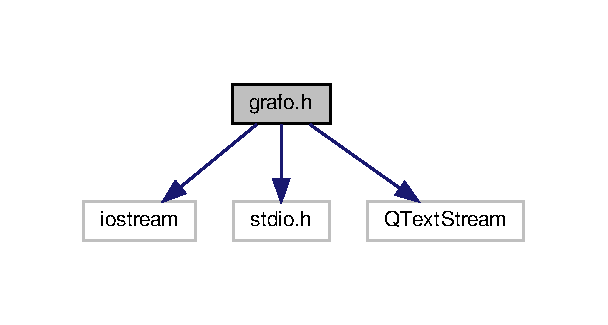
\includegraphics[width=292pt]{grafo_8h__incl}
\end{center}
\end{figure}
This graph shows which files directly or indirectly include this file\+:
\nopagebreak
\begin{figure}[H]
\begin{center}
\leavevmode
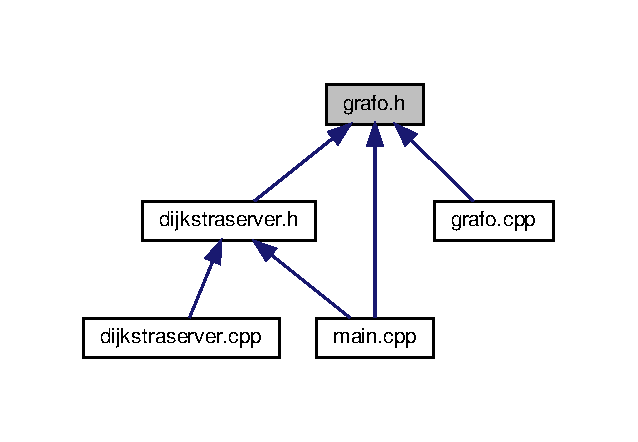
\includegraphics[width=306pt]{grafo_8h__dep__incl}
\end{center}
\end{figure}
\subsection*{Classes}
\begin{DoxyCompactItemize}
\item 
class \hyperlink{class_grafo}{Grafo}
\end{DoxyCompactItemize}
\subsection*{Macros}
\begin{DoxyCompactItemize}
\item 
\#define \hyperlink{grafo_8h_a956e2723d559858d08644ac99146e910}{I\+N\+F\+I\+N\+I\+TY}~9999
\end{DoxyCompactItemize}


\subsection{Detailed Description}
Contiene un grafo y la función Dijkstra. 

\hyperlink{class_grafo}{Grafo} \begin{DoxyVersion}{Version}
1.\+0 
\end{DoxyVersion}
\begin{DoxyAuthor}{Author}
Jose\+Sol 
\end{DoxyAuthor}
\begin{DoxyDate}{Date}
02/03/2020 
\end{DoxyDate}


\subsection{Macro Definition Documentation}
\mbox{\Hypertarget{grafo_8h_a956e2723d559858d08644ac99146e910}\label{grafo_8h_a956e2723d559858d08644ac99146e910}} 
\index{grafo.\+h@{grafo.\+h}!I\+N\+F\+I\+N\+I\+TY@{I\+N\+F\+I\+N\+I\+TY}}
\index{I\+N\+F\+I\+N\+I\+TY@{I\+N\+F\+I\+N\+I\+TY}!grafo.\+h@{grafo.\+h}}
\subsubsection{\texorpdfstring{I\+N\+F\+I\+N\+I\+TY}{INFINITY}}
{\footnotesize\ttfamily \#define I\+N\+F\+I\+N\+I\+TY~9999}


\hypertarget{main_8cpp}{}\section{main.\+cpp File Reference}
\label{main_8cpp}\index{main.\+cpp@{main.\+cpp}}
{\ttfamily \#include $<$Q\+Core\+Application$>$}\newline
{\ttfamily \#include $<$iostream$>$}\newline
{\ttfamily \#include \char`\"{}grafo.\+h\char`\"{}}\newline
{\ttfamily \#include \char`\"{}dijkstraserver.\+h\char`\"{}}\newline
Include dependency graph for main.\+cpp\+:
\nopagebreak
\begin{figure}[H]
\begin{center}
\leavevmode
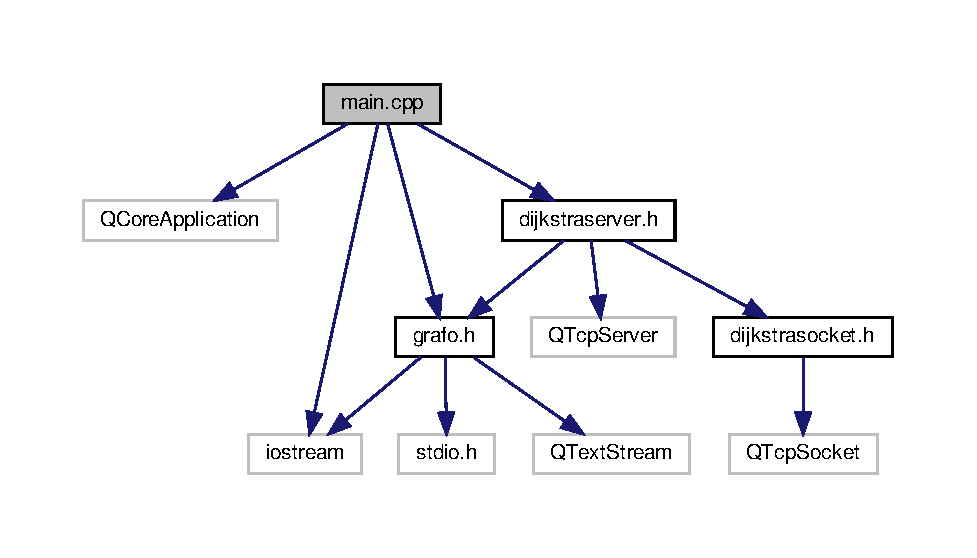
\includegraphics[width=350pt]{main_8cpp__incl}
\end{center}
\end{figure}
\subsection*{Functions}
\begin{DoxyCompactItemize}
\item 
int \hyperlink{main_8cpp_a0ddf1224851353fc92bfbff6f499fa97}{main} (int argc, char $\ast$argv\mbox{[}$\,$\mbox{]})
\end{DoxyCompactItemize}


\subsection{Function Documentation}
\mbox{\Hypertarget{main_8cpp_a0ddf1224851353fc92bfbff6f499fa97}\label{main_8cpp_a0ddf1224851353fc92bfbff6f499fa97}} 
\index{main.\+cpp@{main.\+cpp}!main@{main}}
\index{main@{main}!main.\+cpp@{main.\+cpp}}
\subsubsection{\texorpdfstring{main()}{main()}}
{\footnotesize\ttfamily int main (\begin{DoxyParamCaption}\item[{int}]{argc,  }\item[{char $\ast$}]{argv\mbox{[}$\,$\mbox{]} }\end{DoxyParamCaption})}


\hypertarget{_r_e_a_d_m_e_8md}{}\section{Referencia del Archivo R\+E\+A\+D\+M\+E.\+md}
\label{_r_e_a_d_m_e_8md}\index{R\+E\+A\+D\+M\+E.\+md@{R\+E\+A\+D\+M\+E.\+md}}

%--- End generated contents ---

% Index
\backmatter
\newpage
\phantomsection
\clearemptydoublepage
\addcontentsline{toc}{chapter}{Índice}
\printindex

\end{document}
